\documentclass{if-beamer}
\begin{document}
	
	\title[Campus Formoso do Araguaia]{Matemática Aplicada e noções de Educação financeira}
	\subtitle{Aula 1 }
	\author{Gilmar Gomes do Nascimento}
	\institute[IFTO]{
		Instituto Federal do Tocantins\\
		Campus Formoso do Araguaia
	}
	\date{\today}
	\logo{
		
\includegraphics[scale=0.0085]{logo.jpg}
	}
	\subject{Math} % metadata
	
	\graphicspath{{figuras/}}
	%---------------------------------------------------------------------------------
	\begin{frame}
		\titlepage
	\end{frame}
	\begin{frame}[allowframebreaks]{Economia Solidária}

    \begin{block}{O que é?}
        É um jeito de organizar o trabalho em grupo, onde as próprias trabalhadoras:
        \begin{itemize}
            \item Decidem o que produzir
            \item Definem os preços
            \item Dividem os lucros
            \item Se ajudam mutuamente
        \end{itemize}
    \end{block}

    \framebreak

    \begin{block}{Exemplos}
        \begin{itemize}
            \item Cooperativas de agricultoras
            \item Associações de produtoras
            \item Grupos de venda direta (feiras, delivery)
            \item Fundos de ajuda entre mulheres
        \end{itemize}
    \end{block}

    \framebreak

    \begin{block}{Por que é importante?}
        \begin{itemize}
            \item \textbf{Autonomia:} Sem patrão, a decisão é coletiva
            \item \textbf{Justiça:} O lucro é dividido entre todas
            \item \textbf{Apoio:} Uma ajuda a outra com dinheiro, tempo e ideias
            \item \textbf{Sustentabilidade:} Cuidado com a terra e com as pessoas
        \end{itemize}
    \end{block}

    \framebreak

    \begin{block}{E a horticultura?}
        Muitas feiras orgânicas, cooperativas e associações de produtoras usam 
        esse modelo. É uma forma de vender direto ao consumidor, sem atravessadores,
        e garantir um preço mais justo para quem produz.
    \end{block}

\end{frame}


	\begin{frame}{Revisão Matemática}
		\begin{figure}
			
\includegraphics[scale=0.4]{revisao-matematica}
		\end{figure}		
	\end{frame}
		
	\begin{frame}{Porcentagem}
		\begin{quote}
			Porcentagem é uma forma de expressar uma parte de um todo em relação a 100, representada pelo símbolo \%
		\end{quote}			
	\end{frame}
	
	\begin{frame}[allowframebreaks]{Porcentagem/ponto percentual}
	
	\begin{block}{Distinção}
	 Fique atento para a distinção entre porcentagem e ponto percentual.

Ponto percentual é a diferença, em valores absolutos, entre duas porcentagens.
\framebreak

Uma taxa que passa de 5\% para 10\% aumenta cinco pontos percentuais (10-5=5) ou sobe 100\% (dobra o valor percentual).
\end{block}
	\framebreak
	\begin{block}{}
	Ao comentar a decisão do Comitê de Política Monetária (Copom) do Banco Central de reduzir a taxa de juros em meio ponto percentual, de 12,5\% para 12\%, o senador Eduardo Suplicy (PT-SP) disse que a medida foi consistente e adequada para o Brasil fazer frente à atual crise internacional. 
	\end{block}
	\framebreak
	\begin{block}{Assim não está correto}
	A participação restante será distribuída para estados produtores, na proporção de 20\%; para municípios produtores, na proporção de 4\%; e para municípios afetados por operações de embarque e desembarque, na \textsc{de um ponto percentual}. 	
	\end{block}
	
	\framebreak
	
	\begin{block}{Seria correto}
	A participação restante será distribuída para estados produtores, na proporção de 20\%; para municípios produtores, na proporção de 4\%; e para municípios afetados por operações de embarque e desembarque, na proporção de 1\%. 
	\end{block}
	
	\framebreak
	\begin{block}{Escreva por extenso}
	Outra emenda incluída na Câmara foi o aumento em um ponto percentual do crédito da Cofins recebido pela pessoa jurídica que adquirir tablets fabricados na Zona Franca de Manaus. 
	\end{block}
	
	\framebreak
	\begin{block}{Algarismos}
	Segundo Meirelles, a política monetária tem obtido sucesso na busca da meta de inflação definida para 2004: 5,5\%, com tolerância, para mais ou para menos, de 2,5 pontos percentuais. A expectativa para o fim deste ano, relatou, é de que a inflação alcance 7,3\% — ou 0,7 ponto percentual abaixo do teto definido para 2004, de 8\%. 	
	\end{block}
	
	\framebreak
	
	\begin{block}{}
	Antes, quando a taxa era aumentada em 0,25, 0,5 pontopercentual ou mais, a sociedade se pronunciava, o que era registrado por toda a mídia nacional. Hoje, isso não ocorre, é como diz o ditado popular: ``morreu um gato"~ -- declarou. 
	\end{block}
	
	\end{frame}

	\begin{frame}{Porcentagem}
		\begin{figure}
			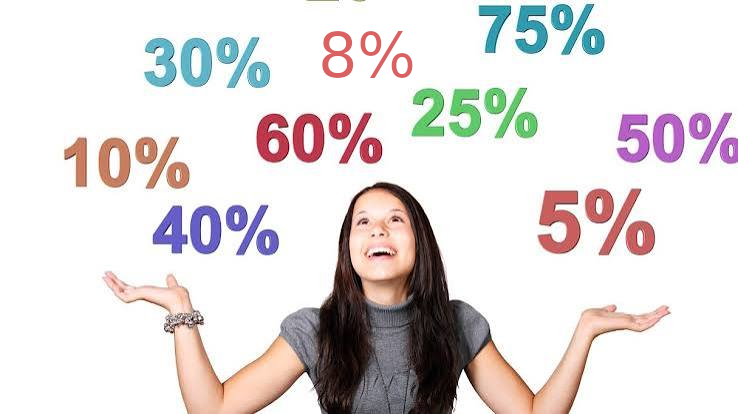
\includegraphics[scale=1.4]{descontos}
		\end{figure}
	\end{frame}
	
	\begin{frame}{Agiotagem é crime?}
	\textbf{Usura} é a prática de cobrar juros excessivos, abusivos ou acima do limite permitido por lei em empréstimos de dinheiro.
	\begin{block}{O que significa?}
		 Agiotagem: É o sinônimo mais comum, conhecido popularmente como a atividade do agiota.Sentido figurado: Também significa ganância, avareza ou apego exagerado ao dinheiro.
	\end{block}	
	\end{frame}
	
	\begin{frame}{Sim, é crime se os juros forem abusivos}
	\begin{itemize}
		\item \textbf{Crime:} A cobrança de juros abusivos é considerada crime contra a economia popular e o sistema financeiro nacional (conhecida como Lei da Usura e Lei dos Crimes contra a Economia Popular).
		\item \textbf{Nulidade:} Contratos que exigem taxas ilegais podem ter cláusulas anuladas ou o valor cobrado em excesso devolvido.
	\end{itemize}
	\end{frame}
	\begin{frame}{Juros simples}
	\centering
	\Huge
	j = c $\times$ i $\times$ t
	\end{frame}		
	
	\begin{frame}{Fórmula do juros simples}
		\begin{center}
			j = c $\times$ i $\times$ t
		\end{center}
		
		j = juros\\
		c = capital \\
		i = taxa \\
		t = tempo
	
	\end{frame}
	
	\begin{frame}[allowframebreaks]{Montante}
	
	\centering
	\Huge
	M = C + J
	
	\framebreak
	
	M = Montante \\
	C = Capital \\
	J = Juros 
	
	\end{frame}
	
	
	\begin{frame}[allowframebreaks]{Introdução aos conceitos de receita}
		\begin{block}{Custo}
			O preço de venda é o valor final pelo qual o produto ou serviço é 
			comercializado com o cliente. Ele é definido a partir do preço de custo, 
			\textbf{acrescido} da margem de lucro que a empresa deseja obter.
		\end{block}
		
		\framebreak
		
		\begin{block}{Exemplo 0. Margem de lucro 15\%}
			Item custa: R\$ 48,00 \\
			Serviço custa: R\$ 30,00
		\end{block}

		\framebreak

		\begin{block}{Desconto}
			O desconto é a diminuição ou o abatimento aplicado sobre o original de um produto, serviço, salário ou dívida. 			
		\end{block}

		\begin{block}{Exemplo 1. Desconto de 12\%}
			Item custa: R\$ 89,90 \\
			Serviço custa: R\$ 140,00
		\end{block}
	\end{frame}	
\end{document}
